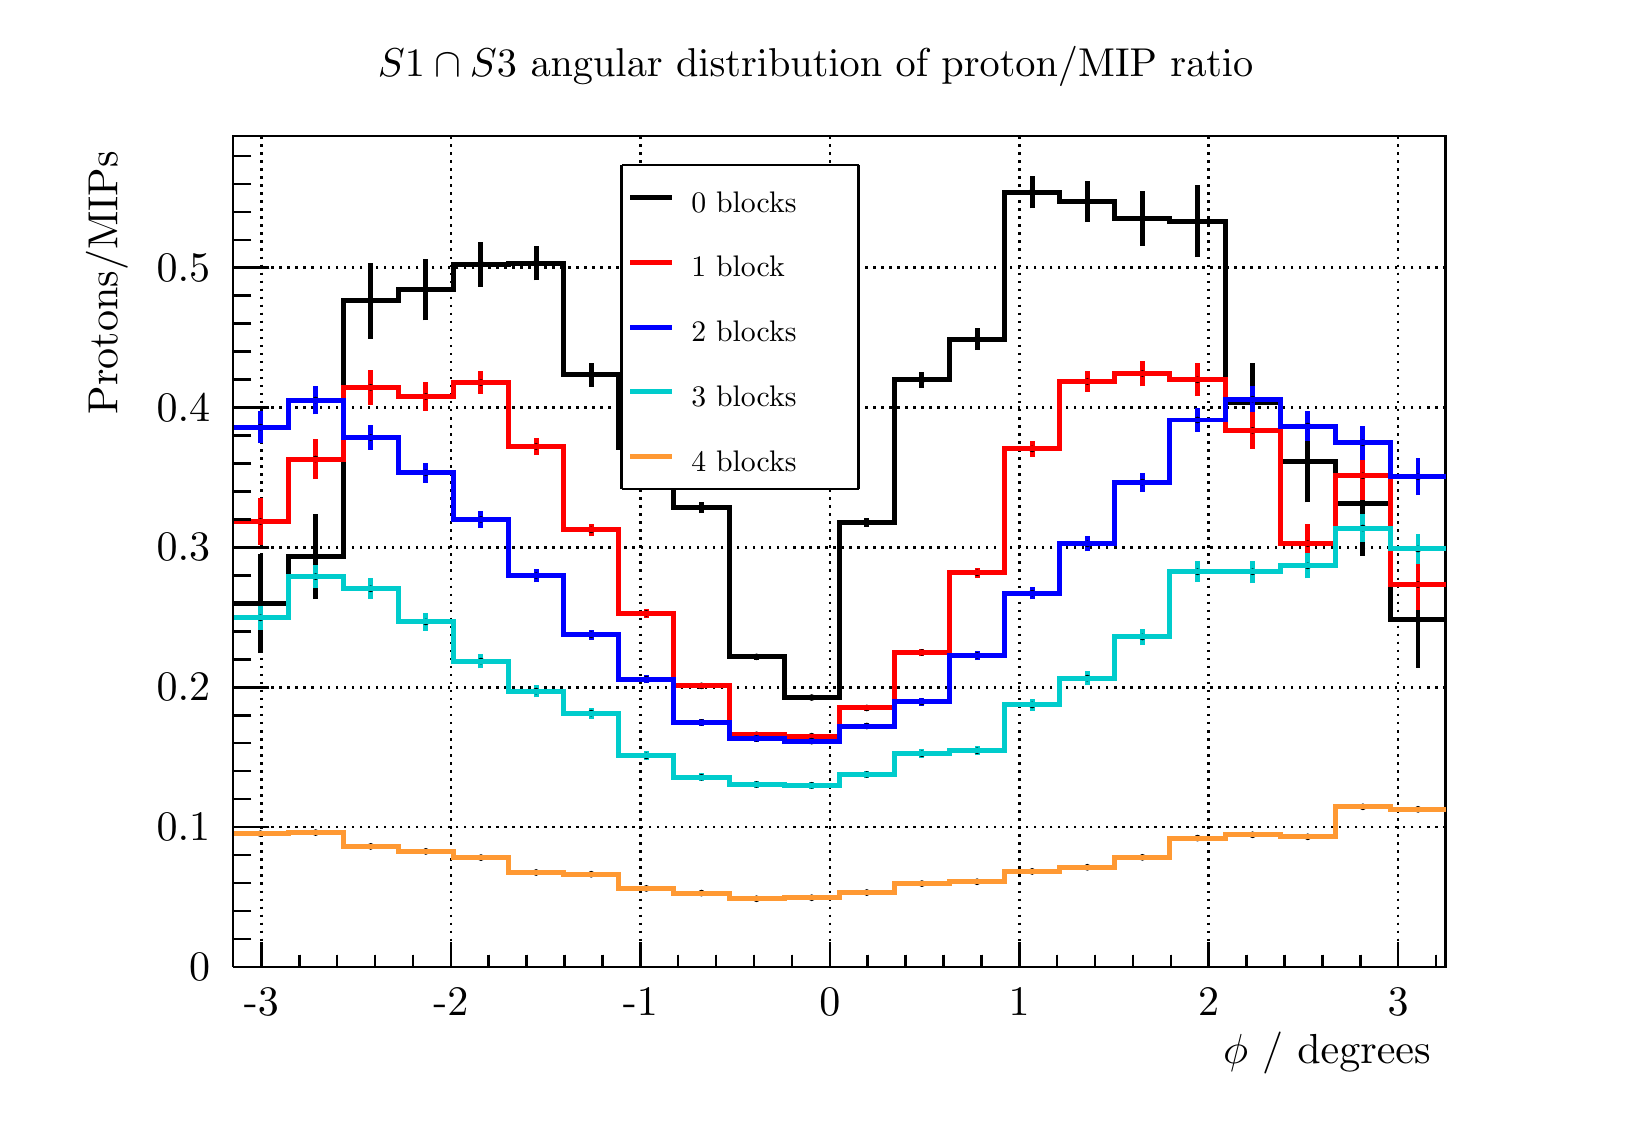
\begin{tikzpicture}
\pgfdeclareplotmark{cross} {
\pgfpathmoveto{\pgfpoint{-0.3\pgfplotmarksize}{\pgfplotmarksize}}
\pgfpathlineto{\pgfpoint{+0.3\pgfplotmarksize}{\pgfplotmarksize}}
\pgfpathlineto{\pgfpoint{+0.3\pgfplotmarksize}{0.3\pgfplotmarksize}}
\pgfpathlineto{\pgfpoint{+1\pgfplotmarksize}{0.3\pgfplotmarksize}}
\pgfpathlineto{\pgfpoint{+1\pgfplotmarksize}{-0.3\pgfplotmarksize}}
\pgfpathlineto{\pgfpoint{+0.3\pgfplotmarksize}{-0.3\pgfplotmarksize}}
\pgfpathlineto{\pgfpoint{+0.3\pgfplotmarksize}{-1.\pgfplotmarksize}}
\pgfpathlineto{\pgfpoint{-0.3\pgfplotmarksize}{-1.\pgfplotmarksize}}
\pgfpathlineto{\pgfpoint{-0.3\pgfplotmarksize}{-0.3\pgfplotmarksize}}
\pgfpathlineto{\pgfpoint{-1.\pgfplotmarksize}{-0.3\pgfplotmarksize}}
\pgfpathlineto{\pgfpoint{-1.\pgfplotmarksize}{0.3\pgfplotmarksize}}
\pgfpathlineto{\pgfpoint{-0.3\pgfplotmarksize}{0.3\pgfplotmarksize}}
\pgfpathclose
\pgfusepathqstroke
}
\pgfdeclareplotmark{cross*} {
\pgfpathmoveto{\pgfpoint{-0.3\pgfplotmarksize}{\pgfplotmarksize}}
\pgfpathlineto{\pgfpoint{+0.3\pgfplotmarksize}{\pgfplotmarksize}}
\pgfpathlineto{\pgfpoint{+0.3\pgfplotmarksize}{0.3\pgfplotmarksize}}
\pgfpathlineto{\pgfpoint{+1\pgfplotmarksize}{0.3\pgfplotmarksize}}
\pgfpathlineto{\pgfpoint{+1\pgfplotmarksize}{-0.3\pgfplotmarksize}}
\pgfpathlineto{\pgfpoint{+0.3\pgfplotmarksize}{-0.3\pgfplotmarksize}}
\pgfpathlineto{\pgfpoint{+0.3\pgfplotmarksize}{-1.\pgfplotmarksize}}
\pgfpathlineto{\pgfpoint{-0.3\pgfplotmarksize}{-1.\pgfplotmarksize}}
\pgfpathlineto{\pgfpoint{-0.3\pgfplotmarksize}{-0.3\pgfplotmarksize}}
\pgfpathlineto{\pgfpoint{-1.\pgfplotmarksize}{-0.3\pgfplotmarksize}}
\pgfpathlineto{\pgfpoint{-1.\pgfplotmarksize}{0.3\pgfplotmarksize}}
\pgfpathlineto{\pgfpoint{-0.3\pgfplotmarksize}{0.3\pgfplotmarksize}}
\pgfpathclose
\pgfusepathqfillstroke
}
\pgfdeclareplotmark{newstar} {
\pgfpathmoveto{\pgfqpoint{0pt}{\pgfplotmarksize}}
\pgfpathlineto{\pgfqpointpolar{44}{0.5\pgfplotmarksize}}
\pgfpathlineto{\pgfqpointpolar{18}{\pgfplotmarksize}}
\pgfpathlineto{\pgfqpointpolar{-20}{0.5\pgfplotmarksize}}
\pgfpathlineto{\pgfqpointpolar{-54}{\pgfplotmarksize}}
\pgfpathlineto{\pgfqpointpolar{-90}{0.5\pgfplotmarksize}}
\pgfpathlineto{\pgfqpointpolar{234}{\pgfplotmarksize}}
\pgfpathlineto{\pgfqpointpolar{198}{0.5\pgfplotmarksize}}
\pgfpathlineto{\pgfqpointpolar{162}{\pgfplotmarksize}}
\pgfpathlineto{\pgfqpointpolar{134}{0.5\pgfplotmarksize}}
\pgfpathclose
\pgfusepathqstroke
}
\pgfdeclareplotmark{newstar*} {
\pgfpathmoveto{\pgfqpoint{0pt}{\pgfplotmarksize}}
\pgfpathlineto{\pgfqpointpolar{44}{0.5\pgfplotmarksize}}
\pgfpathlineto{\pgfqpointpolar{18}{\pgfplotmarksize}}
\pgfpathlineto{\pgfqpointpolar{-20}{0.5\pgfplotmarksize}}
\pgfpathlineto{\pgfqpointpolar{-54}{\pgfplotmarksize}}
\pgfpathlineto{\pgfqpointpolar{-90}{0.5\pgfplotmarksize}}
\pgfpathlineto{\pgfqpointpolar{234}{\pgfplotmarksize}}
\pgfpathlineto{\pgfqpointpolar{198}{0.5\pgfplotmarksize}}
\pgfpathlineto{\pgfqpointpolar{162}{\pgfplotmarksize}}
\pgfpathlineto{\pgfqpointpolar{134}{0.5\pgfplotmarksize}}
\pgfpathclose
\pgfusepathqfillstroke
}
\definecolor{c}{rgb}{1,1,1};
\draw [color=c, fill=c] (0,0) rectangle (20,13.7037);
\draw [color=c, fill=c] (2.6,1.78148) rectangle (18,12.3333);
\definecolor{c}{rgb}{0,0,0};
\draw [c,line width=0.9] (2.6,1.78148) -- (2.6,12.3333) -- (18,12.3333) -- (18,1.78148) -- (2.6,1.78148);
\definecolor{c}{rgb}{1,1,1};
\draw [color=c, fill=c] (2.6,1.78148) rectangle (18,12.3333);
\definecolor{c}{rgb}{0,0,0};
\draw [c,line width=0.9] (2.6,1.78148) -- (2.6,12.3333) -- (18,12.3333) -- (18,1.78148) -- (2.6,1.78148);
\draw [c,line width=0.9] (2.6,1.78148) -- (18,1.78148);
\draw [c,dotted,line width=0.9] (2.96094,12.3333) -- (2.96094,1.78148);
\draw [c,dotted,line width=0.9] (5.36719,12.3333) -- (5.36719,1.78148);
\draw [c,dotted,line width=0.9] (7.77344,12.3333) -- (7.77344,1.78148);
\draw [c,dotted,line width=0.9] (10.1797,12.3333) -- (10.1797,1.78148);
\draw [c,dotted,line width=0.9] (12.5859,12.3333) -- (12.5859,1.78148);
\draw [c,dotted,line width=0.9] (14.9922,12.3333) -- (14.9922,1.78148);
\draw [c,dotted,line width=0.9] (17.3984,12.3333) -- (17.3984,1.78148);
\draw [c,dotted,line width=0.9] (2.96094,12.3333) -- (2.96094,1.78148);
\draw [c,dotted,line width=0.9] (17.3984,12.3333) -- (17.3984,1.78148);
\draw [c,line width=0.9] (2.6,1.78148) -- (2.6,12.3333);
\draw [c,dotted,line width=0.9] (18,1.78148) -- (2.6,1.78148);
\draw [c,dotted,line width=0.9] (18,3.55753) -- (2.6,3.55753);
\draw [c,dotted,line width=0.9] (18,5.33359) -- (2.6,5.33359);
\draw [c,dotted,line width=0.9] (18,7.10964) -- (2.6,7.10964);
\draw [c,dotted,line width=0.9] (18,8.88569) -- (2.6,8.88569);
\draw [c,dotted,line width=0.9] (18,10.6617) -- (2.6,10.6617);
\draw [c,dotted,line width=0.9] (18,10.6617) -- (2.6,10.6617);
\definecolor{c}{rgb}{0,0,0.6};
\draw [c,line width=0.9] (2.6,1.78148) -- (3.3,1.78148) -- (3.3,1.78148) -- (4,1.78148) -- (4,1.78148) -- (4.7,1.78148) -- (4.7,1.78148) -- (5.4,1.78148) -- (5.4,1.78148) -- (6.1,1.78148) -- (6.1,1.78148) -- (6.8,1.78148) -- (6.8,1.78148) --
 (7.5,1.78148) -- (7.5,1.78148) -- (8.2,1.78148) -- (8.2,1.78148) -- (8.9,1.78148) -- (8.9,1.78148) -- (9.6,1.78148) -- (9.6,1.78148) -- (10.3,1.78148) -- (10.3,1.78148) -- (11,1.78148) -- (11,1.78148) -- (11.7,1.78148) -- (11.7,1.78148) --
 (12.4,1.78148) -- (12.4,1.78148) -- (13.1,1.78148) -- (13.1,1.78148) -- (13.8,1.78148) -- (13.8,1.78148) -- (14.5,1.78148) -- (14.5,1.78148) -- (15.2,1.78148) -- (15.2,1.78148) -- (15.9,1.78148) -- (15.9,1.78148) -- (16.6,1.78148) -- (16.6,1.78148)
 -- (17.3,1.78148) -- (17.3,1.78148) -- (18,1.78148);
\definecolor{c}{rgb}{0,0,0};
\draw [c,line width=0.9] (2.6,1.78148) -- (18,1.78148);
\draw [anchor= east] (18,0.685185) node[scale=1.51861, color=c, rotate=0]{$ \phi$ / degrees};
\draw [c,line width=0.9] (2.96094,2.09804) -- (2.96094,1.78148);
\draw [c,line width=0.9] (3.44219,1.93976) -- (3.44219,1.78148);
\draw [c,line width=0.9] (3.92344,1.93976) -- (3.92344,1.78148);
\draw [c,line width=0.9] (4.40469,1.93976) -- (4.40469,1.78148);
\draw [c,line width=0.9] (4.88594,1.93976) -- (4.88594,1.78148);
\draw [c,line width=0.9] (5.36719,2.09804) -- (5.36719,1.78148);
\draw [c,line width=0.9] (5.84844,1.93976) -- (5.84844,1.78148);
\draw [c,line width=0.9] (6.32969,1.93976) -- (6.32969,1.78148);
\draw [c,line width=0.9] (6.81094,1.93976) -- (6.81094,1.78148);
\draw [c,line width=0.9] (7.29219,1.93976) -- (7.29219,1.78148);
\draw [c,line width=0.9] (7.77344,2.09804) -- (7.77344,1.78148);
\draw [c,line width=0.9] (8.25469,1.93976) -- (8.25469,1.78148);
\draw [c,line width=0.9] (8.73594,1.93976) -- (8.73594,1.78148);
\draw [c,line width=0.9] (9.21719,1.93976) -- (9.21719,1.78148);
\draw [c,line width=0.9] (9.69844,1.93976) -- (9.69844,1.78148);
\draw [c,line width=0.9] (10.1797,2.09804) -- (10.1797,1.78148);
\draw [c,line width=0.9] (10.6609,1.93976) -- (10.6609,1.78148);
\draw [c,line width=0.9] (11.1422,1.93976) -- (11.1422,1.78148);
\draw [c,line width=0.9] (11.6234,1.93976) -- (11.6234,1.78148);
\draw [c,line width=0.9] (12.1047,1.93976) -- (12.1047,1.78148);
\draw [c,line width=0.9] (12.5859,2.09804) -- (12.5859,1.78148);
\draw [c,line width=0.9] (13.0672,1.93976) -- (13.0672,1.78148);
\draw [c,line width=0.9] (13.5484,1.93976) -- (13.5484,1.78148);
\draw [c,line width=0.9] (14.0297,1.93976) -- (14.0297,1.78148);
\draw [c,line width=0.9] (14.5109,1.93976) -- (14.5109,1.78148);
\draw [c,line width=0.9] (14.9922,2.09804) -- (14.9922,1.78148);
\draw [c,line width=0.9] (15.4734,1.93976) -- (15.4734,1.78148);
\draw [c,line width=0.9] (15.9547,1.93976) -- (15.9547,1.78148);
\draw [c,line width=0.9] (16.4359,1.93976) -- (16.4359,1.78148);
\draw [c,line width=0.9] (16.9172,1.93976) -- (16.9172,1.78148);
\draw [c,line width=0.9] (17.3984,2.09804) -- (17.3984,1.78148);
\draw [c,line width=0.9] (2.96094,2.09804) -- (2.96094,1.78148);
\draw [c,line width=0.9] (17.3984,2.09804) -- (17.3984,1.78148);
\draw [c,line width=0.9] (17.8797,1.93976) -- (17.8797,1.78148);
\draw [anchor=base] (2.96094,1.16481) node[scale=1.51861, color=c, rotate=0]{-3};
\draw [anchor=base] (5.36719,1.16481) node[scale=1.51861, color=c, rotate=0]{-2};
\draw [anchor=base] (7.77344,1.16481) node[scale=1.51861, color=c, rotate=0]{-1};
\draw [anchor=base] (10.1797,1.16481) node[scale=1.51861, color=c, rotate=0]{0};
\draw [anchor=base] (12.5859,1.16481) node[scale=1.51861, color=c, rotate=0]{1};
\draw [anchor=base] (14.9922,1.16481) node[scale=1.51861, color=c, rotate=0]{2};
\draw [anchor=base] (17.3984,1.16481) node[scale=1.51861, color=c, rotate=0]{3};
\draw [c,line width=0.9] (2.6,1.78148) -- (2.6,12.3333);
\draw [anchor= east] (1,12.3333) node[scale=1.51861, color=c, rotate=90]{  Protons/MIPs};
\draw [c,line width=0.9] (3.062,1.78148) -- (2.6,1.78148);
\draw [c,line width=0.9] (2.831,2.13669) -- (2.6,2.13669);
\draw [c,line width=0.9] (2.831,2.4919) -- (2.6,2.4919);
\draw [c,line width=0.9] (2.831,2.84711) -- (2.6,2.84711);
\draw [c,line width=0.9] (2.831,3.20232) -- (2.6,3.20232);
\draw [c,line width=0.9] (3.062,3.55753) -- (2.6,3.55753);
\draw [c,line width=0.9] (2.831,3.91274) -- (2.6,3.91274);
\draw [c,line width=0.9] (2.831,4.26795) -- (2.6,4.26795);
\draw [c,line width=0.9] (2.831,4.62316) -- (2.6,4.62316);
\draw [c,line width=0.9] (2.831,4.97837) -- (2.6,4.97837);
\draw [c,line width=0.9] (3.062,5.33359) -- (2.6,5.33359);
\draw [c,line width=0.9] (2.831,5.6888) -- (2.6,5.6888);
\draw [c,line width=0.9] (2.831,6.04401) -- (2.6,6.04401);
\draw [c,line width=0.9] (2.831,6.39922) -- (2.6,6.39922);
\draw [c,line width=0.9] (2.831,6.75443) -- (2.6,6.75443);
\draw [c,line width=0.9] (3.062,7.10964) -- (2.6,7.10964);
\draw [c,line width=0.9] (2.831,7.46485) -- (2.6,7.46485);
\draw [c,line width=0.9] (2.831,7.82006) -- (2.6,7.82006);
\draw [c,line width=0.9] (2.831,8.17527) -- (2.6,8.17527);
\draw [c,line width=0.9] (2.831,8.53048) -- (2.6,8.53048);
\draw [c,line width=0.9] (3.062,8.88569) -- (2.6,8.88569);
\draw [c,line width=0.9] (2.831,9.2409) -- (2.6,9.2409);
\draw [c,line width=0.9] (2.831,9.59611) -- (2.6,9.59611);
\draw [c,line width=0.9] (2.831,9.95132) -- (2.6,9.95132);
\draw [c,line width=0.9] (2.831,10.3065) -- (2.6,10.3065);
\draw [c,line width=0.9] (3.062,10.6617) -- (2.6,10.6617);
\draw [c,line width=0.9] (3.062,10.6617) -- (2.6,10.6617);
\draw [c,line width=0.9] (2.831,11.017) -- (2.6,11.017);
\draw [c,line width=0.9] (2.831,11.3722) -- (2.6,11.3722);
\draw [c,line width=0.9] (2.831,11.7274) -- (2.6,11.7274);
\draw [c,line width=0.9] (2.831,12.0826) -- (2.6,12.0826);
\draw [anchor= east] (2.5,1.78148) node[scale=1.51861, color=c, rotate=0]{0};
\draw [anchor= east] (2.5,3.55753) node[scale=1.51861, color=c, rotate=0]{0.1};
\draw [anchor= east] (2.5,5.33359) node[scale=1.51861, color=c, rotate=0]{0.2};
\draw [anchor= east] (2.5,7.10964) node[scale=1.51861, color=c, rotate=0]{0.3};
\draw [anchor= east] (2.5,8.88569) node[scale=1.51861, color=c, rotate=0]{0.4};
\draw [anchor= east] (2.5,10.6617) node[scale=1.51861, color=c, rotate=0]{0.5};
\draw [c,line width=1.8] (2.95,5.76704) -- (2.95,6.3946);
\draw [c,line width=1.8] (2.95,6.3946) -- (2.95,7.02217);
\foreach \P in {(2.95,6.3946)}{\draw[mark options={color=c,fill=c},mark size=2.402402pt,mark=*,mark size=1pt] plot coordinates {\P};}
\draw [c,line width=1.8] (3.65,6.45216) -- (3.65,6.99123);
\draw [c,line width=1.8] (3.65,6.99123) -- (3.65,7.53031);
\foreach \P in {(3.65,6.99123)}{\draw[mark options={color=c,fill=c},mark size=2.402402pt,mark=*,mark size=1pt] plot coordinates {\P};}
\draw [c,line width=1.8] (4.35,9.75889) -- (4.35,10.2414);
\draw [c,line width=1.8] (4.35,10.2414) -- (4.35,10.7239);
\foreach \P in {(4.35,10.2414)}{\draw[mark options={color=c,fill=c},mark size=2.402402pt,mark=*,mark size=1pt] plot coordinates {\P};}
\draw [c,line width=1.8] (5.05,9.99197) -- (5.05,10.3842);
\draw [c,line width=1.8] (5.05,10.3842) -- (5.05,10.7765);
\foreach \P in {(5.05,10.3842)}{\draw[mark options={color=c,fill=c},mark size=2.402402pt,mark=*,mark size=1pt] plot coordinates {\P};}
\draw [c,line width=1.8] (5.75,10.4217) -- (5.75,10.7078);
\draw [c,line width=1.8] (5.75,10.7078) -- (5.75,10.994);
\foreach \P in {(5.75,10.7078)}{\draw[mark options={color=c,fill=c},mark size=2.402402pt,mark=*,mark size=1pt] plot coordinates {\P};}
\draw [c,line width=1.8] (6.45,10.5021) -- (6.45,10.7212);
\draw [c,line width=1.8] (6.45,10.7212) -- (6.45,10.9403);
\foreach \P in {(6.45,10.7212)}{\draw[mark options={color=c,fill=c},mark size=2.402402pt,mark=*,mark size=1pt] plot coordinates {\P};}
\draw [c,line width=1.8] (7.15,9.15002) -- (7.15,9.30123);
\draw [c,line width=1.8] (7.15,9.30123) -- (7.15,9.45244);
\foreach \P in {(7.15,9.30123)}{\draw[mark options={color=c,fill=c},mark size=2.402402pt,mark=*,mark size=1pt] plot coordinates {\P};}
\draw [c,line width=1.8] (7.85,8.27301) -- (7.85,8.37648);
\draw [c,line width=1.8] (7.85,8.37648) -- (7.85,8.47995);
\foreach \P in {(7.85,8.37648)}{\draw[mark options={color=c,fill=c},mark size=2.402402pt,mark=*,mark size=1pt] plot coordinates {\P};}
\draw [c,line width=1.8] (8.55,7.54513) -- (8.55,7.61301);
\draw [c,line width=1.8] (8.55,7.61301) -- (8.55,7.6809);
\foreach \P in {(8.55,7.61301)}{\draw[mark options={color=c,fill=c},mark size=2.402402pt,mark=*,mark size=1pt] plot coordinates {\P};}
\draw [c,line width=1.8] (9.25,5.68523) -- (9.25,5.72005);
\draw [c,line width=1.8] (9.25,5.72005) -- (9.25,5.75486);
\foreach \P in {(9.25,5.72005)}{\draw[mark options={color=c,fill=c},mark size=2.402402pt,mark=*,mark size=1pt] plot coordinates {\P};}
\draw [c,line width=1.8] (9.95,5.17465) -- (9.95,5.20344);
\draw [c,line width=1.8] (9.95,5.20344) -- (9.95,5.23223);
\foreach \P in {(9.95,5.20344)}{\draw[mark options={color=c,fill=c},mark size=2.402402pt,mark=*,mark size=1pt] plot coordinates {\P};}
\draw [c,line width=1.8] (10.65,7.37276) -- (10.65,7.42898);
\draw [c,line width=1.8] (10.65,7.42898) -- (10.65,7.48519);
\foreach \P in {(10.65,7.42898)}{\draw[mark options={color=c,fill=c},mark size=2.402402pt,mark=*,mark size=1pt] plot coordinates {\P};}
\draw [c,line width=1.8] (11.35,9.13744) -- (11.35,9.23629);
\draw [c,line width=1.8] (11.35,9.23629) -- (11.35,9.33514);
\foreach \P in {(11.35,9.23629)}{\draw[mark options={color=c,fill=c},mark size=2.402402pt,mark=*,mark size=1pt] plot coordinates {\P};}
\draw [c,line width=1.8] (12.05,9.61679) -- (12.05,9.75351);
\draw [c,line width=1.8] (12.05,9.75351) -- (12.05,9.89022);
\foreach \P in {(12.05,9.75351)}{\draw[mark options={color=c,fill=c},mark size=2.402402pt,mark=*,mark size=1pt] plot coordinates {\P};}
\draw [c,line width=1.8] (12.75,11.4159) -- (12.75,11.6234);
\draw [c,line width=1.8] (12.75,11.6234) -- (12.75,11.8309);
\foreach \P in {(12.75,11.6234)}{\draw[mark options={color=c,fill=c},mark size=2.402402pt,mark=*,mark size=1pt] plot coordinates {\P};}
\draw [c,line width=1.8] (13.45,11.2397) -- (13.45,11.4998);
\draw [c,line width=1.8] (13.45,11.4998) -- (13.45,11.7599);
\foreach \P in {(13.45,11.4998)}{\draw[mark options={color=c,fill=c},mark size=2.402402pt,mark=*,mark size=1pt] plot coordinates {\P};}
\draw [c,line width=1.8] (14.15,10.9414) -- (14.15,11.2883);
\draw [c,line width=1.8] (14.15,11.2883) -- (14.15,11.6352);
\foreach \P in {(14.15,11.2883)}{\draw[mark options={color=c,fill=c},mark size=2.402402pt,mark=*,mark size=1pt] plot coordinates {\P};}
\draw [c,line width=1.8] (14.85,10.7962) -- (14.85,11.2538);
\draw [c,line width=1.8] (14.85,11.2538) -- (14.85,11.7113);
\foreach \P in {(14.85,11.2538)}{\draw[mark options={color=c,fill=c},mark size=2.402402pt,mark=*,mark size=1pt] plot coordinates {\P};}
\draw [c,line width=1.8] (15.55,8.46064) -- (15.55,8.954);
\draw [c,line width=1.8] (15.55,8.954) -- (15.55,9.44736);
\foreach \P in {(15.55,8.954)}{\draw[mark options={color=c,fill=c},mark size=2.402402pt,mark=*,mark size=1pt] plot coordinates {\P};}
\draw [c,line width=1.8] (16.25,7.68318) -- (16.25,8.1986);
\draw [c,line width=1.8] (16.25,8.1986) -- (16.25,8.71403);
\foreach \P in {(16.25,8.1986)}{\draw[mark options={color=c,fill=c},mark size=2.402402pt,mark=*,mark size=1pt] plot coordinates {\P};}
\draw [c,line width=1.8] (16.95,7.0038) -- (16.95,7.66465);
\draw [c,line width=1.8] (16.95,7.66465) -- (16.95,8.32551);
\foreach \P in {(16.95,7.66465)}{\draw[mark options={color=c,fill=c},mark size=2.402402pt,mark=*,mark size=1pt] plot coordinates {\P};}
\draw [c,line width=1.8] (17.65,5.58087) -- (17.65,6.19333);
\draw [c,line width=1.8] (17.65,6.19333) -- (17.65,6.80579);
\foreach \P in {(17.65,6.19333)}{\draw[mark options={color=c,fill=c},mark size=2.402402pt,mark=*,mark size=1pt] plot coordinates {\P};}
\draw [c,line width=1.8] (2.6,6.3946) -- (3.3,6.3946) -- (3.3,6.99123) -- (4,6.99123) -- (4,10.2414) -- (4.7,10.2414) -- (4.7,10.3842) -- (5.4,10.3842) -- (5.4,10.7078) -- (6.1,10.7078) -- (6.1,10.7212) -- (6.8,10.7212) -- (6.8,9.30123) --
 (7.5,9.30123) -- (7.5,8.37648) -- (8.2,8.37648) -- (8.2,7.61301) -- (8.9,7.61301) -- (8.9,5.72005) -- (9.6,5.72005) -- (9.6,5.20344) -- (10.3,5.20344) -- (10.3,7.42898) -- (11,7.42898) -- (11,9.23629) -- (11.7,9.23629) -- (11.7,9.75351) --
 (12.4,9.75351) -- (12.4,11.6234) -- (13.1,11.6234) -- (13.1,11.4998) -- (13.8,11.4998) -- (13.8,11.2883) -- (14.5,11.2883) -- (14.5,11.2538) -- (15.2,11.2538) -- (15.2,8.954) -- (15.9,8.954) -- (15.9,8.1986) -- (16.6,8.1986) -- (16.6,7.66465) --
 (17.3,7.66465) -- (17.3,6.19333) -- (18,6.19333);
\definecolor{c}{rgb}{1,0,0};
\draw [c,line width=1.8] (2.95,7.14547) -- (2.95,7.4397);
\draw [c,line width=1.8] (2.95,7.4397) -- (2.95,7.73393);
\definecolor{c}{rgb}{0,0,0};
\foreach \P in {(2.95,7.4397)}{\draw[mark options={color=c,fill=c},mark size=2.402402pt,mark=*,mark size=1pt] plot coordinates {\P};}
\definecolor{c}{rgb}{1,0,0};
\draw [c,line width=1.8] (3.65,7.97681) -- (3.65,8.23261);
\draw [c,line width=1.8] (3.65,8.23261) -- (3.65,8.48841);
\definecolor{c}{rgb}{0,0,0};
\foreach \P in {(3.65,8.23261)}{\draw[mark options={color=c,fill=c},mark size=2.402402pt,mark=*,mark size=1pt] plot coordinates {\P};}
\definecolor{c}{rgb}{1,0,0};
\draw [c,line width=1.8] (4.35,8.91713) -- (4.35,9.14244);
\draw [c,line width=1.8] (4.35,9.14244) -- (4.35,9.36775);
\definecolor{c}{rgb}{0,0,0};
\foreach \P in {(4.35,9.14244)}{\draw[mark options={color=c,fill=c},mark size=2.402402pt,mark=*,mark size=1pt] plot coordinates {\P};}
\definecolor{c}{rgb}{1,0,0};
\draw [c,line width=1.8] (5.05,8.84546) -- (5.05,9.02691);
\draw [c,line width=1.8] (5.05,9.02691) -- (5.05,9.20836);
\definecolor{c}{rgb}{0,0,0};
\foreach \P in {(5.05,9.02691)}{\draw[mark options={color=c,fill=c},mark size=2.402402pt,mark=*,mark size=1pt] plot coordinates {\P};}
\definecolor{c}{rgb}{1,0,0};
\draw [c,line width=1.8] (5.75,9.05915) -- (5.75,9.20336);
\draw [c,line width=1.8] (5.75,9.20336) -- (5.75,9.34756);
\definecolor{c}{rgb}{0,0,0};
\foreach \P in {(5.75,9.20336)}{\draw[mark options={color=c,fill=c},mark size=2.402402pt,mark=*,mark size=1pt] plot coordinates {\P};}
\definecolor{c}{rgb}{1,0,0};
\draw [c,line width=1.8] (6.45,8.2807) -- (6.45,8.39163);
\draw [c,line width=1.8] (6.45,8.39163) -- (6.45,8.50257);
\definecolor{c}{rgb}{0,0,0};
\foreach \P in {(6.45,8.39163)}{\draw[mark options={color=c,fill=c},mark size=2.402402pt,mark=*,mark size=1pt] plot coordinates {\P};}
\definecolor{c}{rgb}{1,0,0};
\draw [c,line width=1.8] (7.15,7.25321) -- (7.15,7.33278);
\draw [c,line width=1.8] (7.15,7.33278) -- (7.15,7.41235);
\definecolor{c}{rgb}{0,0,0};
\foreach \P in {(7.15,7.33278)}{\draw[mark options={color=c,fill=c},mark size=2.402402pt,mark=*,mark size=1pt] plot coordinates {\P};}
\definecolor{c}{rgb}{1,0,0};
\draw [c,line width=1.8] (7.85,6.21588) -- (7.85,6.27281);
\draw [c,line width=1.8] (7.85,6.27281) -- (7.85,6.32975);
\definecolor{c}{rgb}{0,0,0};
\foreach \P in {(7.85,6.27281)}{\draw[mark options={color=c,fill=c},mark size=2.402402pt,mark=*,mark size=1pt] plot coordinates {\P};}
\definecolor{c}{rgb}{1,0,0};
\draw [c,line width=1.8] (8.55,5.31013) -- (8.55,5.35218);
\draw [c,line width=1.8] (8.55,5.35218) -- (8.55,5.39422);
\definecolor{c}{rgb}{0,0,0};
\foreach \P in {(8.55,5.35218)}{\draw[mark options={color=c,fill=c},mark size=2.402402pt,mark=*,mark size=1pt] plot coordinates {\P};}
\definecolor{c}{rgb}{1,0,0};
\draw [c,line width=1.8] (9.25,4.69635) -- (9.25,4.73012);
\draw [c,line width=1.8] (9.25,4.73012) -- (9.25,4.7639);
\definecolor{c}{rgb}{0,0,0};
\foreach \P in {(9.25,4.73012)}{\draw[mark options={color=c,fill=c},mark size=2.402402pt,mark=*,mark size=1pt] plot coordinates {\P};}
\definecolor{c}{rgb}{1,0,0};
\draw [c,line width=1.8] (9.95,4.68001) -- (9.95,4.71315);
\draw [c,line width=1.8] (9.95,4.71315) -- (9.95,4.74629);
\definecolor{c}{rgb}{0,0,0};
\foreach \P in {(9.95,4.71315)}{\draw[mark options={color=c,fill=c},mark size=2.402402pt,mark=*,mark size=1pt] plot coordinates {\P};}
\definecolor{c}{rgb}{1,0,0};
\draw [c,line width=1.8] (10.65,5.03329) -- (10.65,5.07106);
\draw [c,line width=1.8] (10.65,5.07106) -- (10.65,5.10883);
\definecolor{c}{rgb}{0,0,0};
\foreach \P in {(10.65,5.07106)}{\draw[mark options={color=c,fill=c},mark size=2.402402pt,mark=*,mark size=1pt] plot coordinates {\P};}
\definecolor{c}{rgb}{1,0,0};
\draw [c,line width=1.8] (11.35,5.72715) -- (11.35,5.77577);
\draw [c,line width=1.8] (11.35,5.77577) -- (11.35,5.82438);
\definecolor{c}{rgb}{0,0,0};
\foreach \P in {(11.35,5.77577)}{\draw[mark options={color=c,fill=c},mark size=2.402402pt,mark=*,mark size=1pt] plot coordinates {\P};}
\definecolor{c}{rgb}{1,0,0};
\draw [c,line width=1.8] (12.05,6.72143) -- (12.05,6.78741);
\draw [c,line width=1.8] (12.05,6.78741) -- (12.05,6.85339);
\definecolor{c}{rgb}{0,0,0};
\foreach \P in {(12.05,6.78741)}{\draw[mark options={color=c,fill=c},mark size=2.402402pt,mark=*,mark size=1pt] plot coordinates {\P};}
\definecolor{c}{rgb}{1,0,0};
\draw [c,line width=1.8] (12.75,8.26167) -- (12.75,8.36122);
\draw [c,line width=1.8] (12.75,8.36122) -- (12.75,8.46078);
\definecolor{c}{rgb}{0,0,0};
\foreach \P in {(12.75,8.36122)}{\draw[mark options={color=c,fill=c},mark size=2.402402pt,mark=*,mark size=1pt] plot coordinates {\P};}
\definecolor{c}{rgb}{1,0,0};
\draw [c,line width=1.8] (13.45,9.08493) -- (13.45,9.2163);
\draw [c,line width=1.8] (13.45,9.2163) -- (13.45,9.34768);
\definecolor{c}{rgb}{0,0,0};
\foreach \P in {(13.45,9.2163)}{\draw[mark options={color=c,fill=c},mark size=2.402402pt,mark=*,mark size=1pt] plot coordinates {\P};}
\definecolor{c}{rgb}{1,0,0};
\draw [c,line width=1.8] (14.15,9.1541) -- (14.15,9.3189);
\draw [c,line width=1.8] (14.15,9.3189) -- (14.15,9.48371);
\definecolor{c}{rgb}{0,0,0};
\foreach \P in {(14.15,9.3189)}{\draw[mark options={color=c,fill=c},mark size=2.402402pt,mark=*,mark size=1pt] plot coordinates {\P};}
\definecolor{c}{rgb}{1,0,0};
\draw [c,line width=1.8] (14.85,9.02994) -- (14.85,9.23888);
\draw [c,line width=1.8] (14.85,9.23888) -- (14.85,9.44782);
\definecolor{c}{rgb}{0,0,0};
\foreach \P in {(14.85,9.23888)}{\draw[mark options={color=c,fill=c},mark size=2.402402pt,mark=*,mark size=1pt] plot coordinates {\P};}
\definecolor{c}{rgb}{1,0,0};
\draw [c,line width=1.8] (15.55,8.3612) -- (15.55,8.59626);
\draw [c,line width=1.8] (15.55,8.59626) -- (15.55,8.83132);
\definecolor{c}{rgb}{0,0,0};
\foreach \P in {(15.55,8.59626)}{\draw[mark options={color=c,fill=c},mark size=2.402402pt,mark=*,mark size=1pt] plot coordinates {\P};}
\definecolor{c}{rgb}{1,0,0};
\draw [c,line width=1.8] (16.25,6.91205) -- (16.25,7.15808);
\draw [c,line width=1.8] (16.25,7.15808) -- (16.25,7.4041);
\definecolor{c}{rgb}{0,0,0};
\foreach \P in {(16.25,7.15808)}{\draw[mark options={color=c,fill=c},mark size=2.402402pt,mark=*,mark size=1pt] plot coordinates {\P};}
\definecolor{c}{rgb}{1,0,0};
\draw [c,line width=1.8] (16.95,7.71285) -- (16.95,8.01978);
\draw [c,line width=1.8] (16.95,8.01978) -- (16.95,8.32671);
\definecolor{c}{rgb}{0,0,0};
\foreach \P in {(16.95,8.01978)}{\draw[mark options={color=c,fill=c},mark size=2.402402pt,mark=*,mark size=1pt] plot coordinates {\P};}
\definecolor{c}{rgb}{1,0,0};
\draw [c,line width=1.8] (17.65,6.31987) -- (17.65,6.63832);
\draw [c,line width=1.8] (17.65,6.63832) -- (17.65,6.95677);
\definecolor{c}{rgb}{0,0,0};
\foreach \P in {(17.65,6.63832)}{\draw[mark options={color=c,fill=c},mark size=2.402402pt,mark=*,mark size=1pt] plot coordinates {\P};}
\definecolor{c}{rgb}{1,0,0};
\draw [c,line width=1.8] (2.6,7.4397) -- (3.3,7.4397) -- (3.3,8.23261) -- (4,8.23261) -- (4,9.14244) -- (4.7,9.14244) -- (4.7,9.02691) -- (5.4,9.02691) -- (5.4,9.20336) -- (6.1,9.20336) -- (6.1,8.39163) -- (6.8,8.39163) -- (6.8,7.33278) --
 (7.5,7.33278) -- (7.5,6.27281) -- (8.2,6.27281) -- (8.2,5.35218) -- (8.9,5.35218) -- (8.9,4.73012) -- (9.6,4.73012) -- (9.6,4.71315) -- (10.3,4.71315) -- (10.3,5.07106) -- (11,5.07106) -- (11,5.77577) -- (11.7,5.77577) -- (11.7,6.78741) --
 (12.4,6.78741) -- (12.4,8.36122) -- (13.1,8.36122) -- (13.1,9.2163) -- (13.8,9.2163) -- (13.8,9.3189) -- (14.5,9.3189) -- (14.5,9.23888) -- (15.2,9.23888) -- (15.2,8.59626) -- (15.9,8.59626) -- (15.9,7.15808) -- (16.6,7.15808) -- (16.6,8.01978) --
 (17.3,8.01978) -- (17.3,6.63832) -- (18,6.63832);
\definecolor{c}{rgb}{0,0,1};
\draw [c,line width=1.8] (2.95,8.43327) -- (2.95,8.63764);
\draw [c,line width=1.8] (2.95,8.63764) -- (2.95,8.84201);
\definecolor{c}{rgb}{0,0,0};
\foreach \P in {(2.95,8.63764)}{\draw[mark options={color=c,fill=c},mark size=2.402402pt,mark=*,mark size=1pt] plot coordinates {\P};}
\definecolor{c}{rgb}{0,0,1};
\draw [c,line width=1.8] (3.65,8.80108) -- (3.65,8.98169);
\draw [c,line width=1.8] (3.65,8.98169) -- (3.65,9.1623);
\definecolor{c}{rgb}{0,0,0};
\foreach \P in {(3.65,8.98169)}{\draw[mark options={color=c,fill=c},mark size=2.402402pt,mark=*,mark size=1pt] plot coordinates {\P};}
\definecolor{c}{rgb}{0,0,1};
\draw [c,line width=1.8] (4.35,8.35147) -- (4.35,8.50584);
\draw [c,line width=1.8] (4.35,8.50584) -- (4.35,8.66021);
\definecolor{c}{rgb}{0,0,0};
\foreach \P in {(4.35,8.50584)}{\draw[mark options={color=c,fill=c},mark size=2.402402pt,mark=*,mark size=1pt] plot coordinates {\P};}
\definecolor{c}{rgb}{0,0,1};
\draw [c,line width=1.8] (5.05,7.92955) -- (5.05,8.05859);
\draw [c,line width=1.8] (5.05,8.05859) -- (5.05,8.18763);
\definecolor{c}{rgb}{0,0,0};
\foreach \P in {(5.05,8.05859)}{\draw[mark options={color=c,fill=c},mark size=2.402402pt,mark=*,mark size=1pt] plot coordinates {\P};}
\definecolor{c}{rgb}{0,0,1};
\draw [c,line width=1.8] (5.75,7.3623) -- (5.75,7.46585);
\draw [c,line width=1.8] (5.75,7.46585) -- (5.75,7.5694);
\definecolor{c}{rgb}{0,0,0};
\foreach \P in {(5.75,7.46585)}{\draw[mark options={color=c,fill=c},mark size=2.402402pt,mark=*,mark size=1pt] plot coordinates {\P};}
\definecolor{c}{rgb}{0,0,1};
\draw [c,line width=1.8] (6.45,6.66742) -- (6.45,6.75233);
\draw [c,line width=1.8] (6.45,6.75233) -- (6.45,6.83724);
\definecolor{c}{rgb}{0,0,0};
\foreach \P in {(6.45,6.75233)}{\draw[mark options={color=c,fill=c},mark size=2.402402pt,mark=*,mark size=1pt] plot coordinates {\P};}
\definecolor{c}{rgb}{0,0,1};
\draw [c,line width=1.8] (7.15,5.93444) -- (7.15,6.00054);
\draw [c,line width=1.8] (7.15,6.00054) -- (7.15,6.06664);
\definecolor{c}{rgb}{0,0,0};
\foreach \P in {(7.15,6.00054)}{\draw[mark options={color=c,fill=c},mark size=2.402402pt,mark=*,mark size=1pt] plot coordinates {\P};}
\definecolor{c}{rgb}{0,0,1};
\draw [c,line width=1.8] (7.85,5.38383) -- (7.85,5.43728);
\draw [c,line width=1.8] (7.85,5.43728) -- (7.85,5.49072);
\definecolor{c}{rgb}{0,0,0};
\foreach \P in {(7.85,5.43728)}{\draw[mark options={color=c,fill=c},mark size=2.402402pt,mark=*,mark size=1pt] plot coordinates {\P};}
\definecolor{c}{rgb}{0,0,1};
\draw [c,line width=1.8] (8.55,4.84367) -- (8.55,4.888);
\draw [c,line width=1.8] (8.55,4.888) -- (8.55,4.93233);
\definecolor{c}{rgb}{0,0,0};
\foreach \P in {(8.55,4.888)}{\draw[mark options={color=c,fill=c},mark size=2.402402pt,mark=*,mark size=1pt] plot coordinates {\P};}
\definecolor{c}{rgb}{0,0,1};
\draw [c,line width=1.8] (9.25,4.64316) -- (9.25,4.68321);
\draw [c,line width=1.8] (9.25,4.68321) -- (9.25,4.72326);
\definecolor{c}{rgb}{0,0,0};
\foreach \P in {(9.25,4.68321)}{\draw[mark options={color=c,fill=c},mark size=2.402402pt,mark=*,mark size=1pt] plot coordinates {\P};}
\definecolor{c}{rgb}{0,0,1};
\draw [c,line width=1.8] (9.95,4.60912) -- (9.95,4.64921);
\draw [c,line width=1.8] (9.95,4.64921) -- (9.95,4.6893);
\definecolor{c}{rgb}{0,0,0};
\foreach \P in {(9.95,4.64921)}{\draw[mark options={color=c,fill=c},mark size=2.402402pt,mark=*,mark size=1pt] plot coordinates {\P};}
\definecolor{c}{rgb}{0,0,1};
\draw [c,line width=1.8] (10.65,4.79856) -- (10.65,4.84146);
\draw [c,line width=1.8] (10.65,4.84146) -- (10.65,4.88436);
\definecolor{c}{rgb}{0,0,0};
\foreach \P in {(10.65,4.84146)}{\draw[mark options={color=c,fill=c},mark size=2.402402pt,mark=*,mark size=1pt] plot coordinates {\P};}
\definecolor{c}{rgb}{0,0,1};
\draw [c,line width=1.8] (11.35,5.09841) -- (11.35,5.14734);
\draw [c,line width=1.8] (11.35,5.14734) -- (11.35,5.19628);
\definecolor{c}{rgb}{0,0,0};
\foreach \P in {(11.35,5.14734)}{\draw[mark options={color=c,fill=c},mark size=2.402402pt,mark=*,mark size=1pt] plot coordinates {\P};}
\definecolor{c}{rgb}{0,0,1};
\draw [c,line width=1.8] (12.05,5.67929) -- (12.05,5.73854);
\draw [c,line width=1.8] (12.05,5.73854) -- (12.05,5.79778);
\definecolor{c}{rgb}{0,0,0};
\foreach \P in {(12.05,5.73854)}{\draw[mark options={color=c,fill=c},mark size=2.402402pt,mark=*,mark size=1pt] plot coordinates {\P};}
\definecolor{c}{rgb}{0,0,1};
\draw [c,line width=1.8] (12.75,6.45139) -- (12.75,6.52907);
\draw [c,line width=1.8] (12.75,6.52907) -- (12.75,6.60675);
\definecolor{c}{rgb}{0,0,0};
\foreach \P in {(12.75,6.52907)}{\draw[mark options={color=c,fill=c},mark size=2.402402pt,mark=*,mark size=1pt] plot coordinates {\P};}
\definecolor{c}{rgb}{0,0,1};
\draw [c,line width=1.8] (13.45,7.05859) -- (13.45,7.15536);
\draw [c,line width=1.8] (13.45,7.15536) -- (13.45,7.25212);
\definecolor{c}{rgb}{0,0,0};
\foreach \P in {(13.45,7.15536)}{\draw[mark options={color=c,fill=c},mark size=2.402402pt,mark=*,mark size=1pt] plot coordinates {\P};}
\definecolor{c}{rgb}{0,0,1};
\draw [c,line width=1.8] (14.15,7.81939) -- (14.15,7.93908);
\draw [c,line width=1.8] (14.15,7.93908) -- (14.15,8.05877);
\definecolor{c}{rgb}{0,0,0};
\foreach \P in {(14.15,7.93908)}{\draw[mark options={color=c,fill=c},mark size=2.402402pt,mark=*,mark size=1pt] plot coordinates {\P};}
\definecolor{c}{rgb}{0,0,1};
\draw [c,line width=1.8] (14.85,8.58105) -- (14.85,8.72814);
\draw [c,line width=1.8] (14.85,8.72814) -- (14.85,8.87523);
\definecolor{c}{rgb}{0,0,0};
\foreach \P in {(14.85,8.72814)}{\draw[mark options={color=c,fill=c},mark size=2.402402pt,mark=*,mark size=1pt] plot coordinates {\P};}
\definecolor{c}{rgb}{0,0,1};
\draw [c,line width=1.8] (15.55,8.82447) -- (15.55,8.99257);
\draw [c,line width=1.8] (15.55,8.99257) -- (15.55,9.16067);
\definecolor{c}{rgb}{0,0,0};
\foreach \P in {(15.55,8.99257)}{\draw[mark options={color=c,fill=c},mark size=2.402402pt,mark=*,mark size=1pt] plot coordinates {\P};}
\definecolor{c}{rgb}{0,0,1};
\draw [c,line width=1.8] (16.25,8.46545) -- (16.25,8.65174);
\draw [c,line width=1.8] (16.25,8.65174) -- (16.25,8.83803);
\definecolor{c}{rgb}{0,0,0};
\foreach \P in {(16.25,8.65174)}{\draw[mark options={color=c,fill=c},mark size=2.402402pt,mark=*,mark size=1pt] plot coordinates {\P};}
\definecolor{c}{rgb}{0,0,1};
\draw [c,line width=1.8] (16.95,8.21985) -- (16.95,8.4388);
\draw [c,line width=1.8] (16.95,8.4388) -- (16.95,8.65774);
\definecolor{c}{rgb}{0,0,0};
\foreach \P in {(16.95,8.4388)}{\draw[mark options={color=c,fill=c},mark size=2.402402pt,mark=*,mark size=1pt] plot coordinates {\P};}
\definecolor{c}{rgb}{0,0,1};
\draw [c,line width=1.8] (17.65,7.77367) -- (17.65,8.0071);
\draw [c,line width=1.8] (17.65,8.0071) -- (17.65,8.24052);
\definecolor{c}{rgb}{0,0,0};
\foreach \P in {(17.65,8.0071)}{\draw[mark options={color=c,fill=c},mark size=2.402402pt,mark=*,mark size=1pt] plot coordinates {\P};}
\definecolor{c}{rgb}{0,0,1};
\draw [c,line width=1.8] (2.6,8.63764) -- (3.3,8.63764) -- (3.3,8.98169) -- (4,8.98169) -- (4,8.50584) -- (4.7,8.50584) -- (4.7,8.05859) -- (5.4,8.05859) -- (5.4,7.46585) -- (6.1,7.46585) -- (6.1,6.75233) -- (6.8,6.75233) -- (6.8,6.00054) --
 (7.5,6.00054) -- (7.5,5.43728) -- (8.2,5.43728) -- (8.2,4.888) -- (8.9,4.888) -- (8.9,4.68321) -- (9.6,4.68321) -- (9.6,4.64921) -- (10.3,4.64921) -- (10.3,4.84146) -- (11,4.84146) -- (11,5.14734) -- (11.7,5.14734) -- (11.7,5.73854) --
 (12.4,5.73854) -- (12.4,6.52907) -- (13.1,6.52907) -- (13.1,7.15536) -- (13.8,7.15536) -- (13.8,7.93908) -- (14.5,7.93908) -- (14.5,8.72814) -- (15.2,8.72814) -- (15.2,8.99257) -- (15.9,8.99257) -- (15.9,8.65174) -- (16.6,8.65174) -- (16.6,8.4388)
 -- (17.3,8.4388) -- (17.3,8.0071) -- (18,8.0071);
\definecolor{c}{rgb}{0,0.8,0.8};
\draw [c,line width=1.8] (2.95,6.06144) -- (2.95,6.21621);
\draw [c,line width=1.8] (2.95,6.21621) -- (2.95,6.37099);
\definecolor{c}{rgb}{0,0,0};
\foreach \P in {(2.95,6.21621)}{\draw[mark options={color=c,fill=c},mark size=2.402402pt,mark=*,mark size=1pt] plot coordinates {\P};}
\definecolor{c}{rgb}{0,0.8,0.8};
\draw [c,line width=1.8] (3.65,6.58978) -- (3.65,6.73877);
\draw [c,line width=1.8] (3.65,6.73877) -- (3.65,6.88777);
\definecolor{c}{rgb}{0,0,0};
\foreach \P in {(3.65,6.73877)}{\draw[mark options={color=c,fill=c},mark size=2.402402pt,mark=*,mark size=1pt] plot coordinates {\P};}
\definecolor{c}{rgb}{0,0.8,0.8};
\draw [c,line width=1.8] (4.35,6.45258) -- (4.35,6.58458);
\draw [c,line width=1.8] (4.35,6.58458) -- (4.35,6.71658);
\definecolor{c}{rgb}{0,0,0};
\foreach \P in {(4.35,6.58458)}{\draw[mark options={color=c,fill=c},mark size=2.402402pt,mark=*,mark size=1pt] plot coordinates {\P};}
\definecolor{c}{rgb}{0,0.8,0.8};
\draw [c,line width=1.8] (5.05,6.0507) -- (5.05,6.16365);
\draw [c,line width=1.8] (5.05,6.16365) -- (5.05,6.27659);
\definecolor{c}{rgb}{0,0,0};
\foreach \P in {(5.05,6.16365)}{\draw[mark options={color=c,fill=c},mark size=2.402402pt,mark=*,mark size=1pt] plot coordinates {\P};}
\definecolor{c}{rgb}{0,0.8,0.8};
\draw [c,line width=1.8] (5.75,5.57341) -- (5.75,5.6666);
\draw [c,line width=1.8] (5.75,5.6666) -- (5.75,5.75978);
\definecolor{c}{rgb}{0,0,0};
\foreach \P in {(5.75,5.6666)}{\draw[mark options={color=c,fill=c},mark size=2.402402pt,mark=*,mark size=1pt] plot coordinates {\P};}
\definecolor{c}{rgb}{0,0.8,0.8};
\draw [c,line width=1.8] (6.45,5.20417) -- (6.45,5.28534);
\draw [c,line width=1.8] (6.45,5.28534) -- (6.45,5.3665);
\definecolor{c}{rgb}{0,0,0};
\foreach \P in {(6.45,5.28534)}{\draw[mark options={color=c,fill=c},mark size=2.402402pt,mark=*,mark size=1pt] plot coordinates {\P};}
\definecolor{c}{rgb}{0,0.8,0.8};
\draw [c,line width=1.8] (7.15,4.93568) -- (7.15,5.00532);
\draw [c,line width=1.8] (7.15,5.00532) -- (7.15,5.07496);
\definecolor{c}{rgb}{0,0,0};
\foreach \P in {(7.15,5.00532)}{\draw[mark options={color=c,fill=c},mark size=2.402402pt,mark=*,mark size=1pt] plot coordinates {\P};}
\definecolor{c}{rgb}{0,0.8,0.8};
\draw [c,line width=1.8] (7.85,4.40576) -- (7.85,4.46224);
\draw [c,line width=1.8] (7.85,4.46224) -- (7.85,4.51871);
\definecolor{c}{rgb}{0,0,0};
\foreach \P in {(7.85,4.46224)}{\draw[mark options={color=c,fill=c},mark size=2.402402pt,mark=*,mark size=1pt] plot coordinates {\P};}
\definecolor{c}{rgb}{0,0.8,0.8};
\draw [c,line width=1.8] (8.55,4.14083) -- (8.55,4.19093);
\draw [c,line width=1.8] (8.55,4.19093) -- (8.55,4.24104);
\definecolor{c}{rgb}{0,0,0};
\foreach \P in {(8.55,4.19093)}{\draw[mark options={color=c,fill=c},mark size=2.402402pt,mark=*,mark size=1pt] plot coordinates {\P};}
\definecolor{c}{rgb}{0,0.8,0.8};
\draw [c,line width=1.8] (9.25,4.05201) -- (9.25,4.09902);
\draw [c,line width=1.8] (9.25,4.09902) -- (9.25,4.14604);
\definecolor{c}{rgb}{0,0,0};
\foreach \P in {(9.25,4.09902)}{\draw[mark options={color=c,fill=c},mark size=2.402402pt,mark=*,mark size=1pt] plot coordinates {\P};}
\definecolor{c}{rgb}{0,0.8,0.8};
\draw [c,line width=1.8] (9.95,4.04153) -- (9.95,4.08854);
\draw [c,line width=1.8] (9.95,4.08854) -- (9.95,4.13556);
\definecolor{c}{rgb}{0,0,0};
\foreach \P in {(9.95,4.08854)}{\draw[mark options={color=c,fill=c},mark size=2.402402pt,mark=*,mark size=1pt] plot coordinates {\P};}
\definecolor{c}{rgb}{0,0.8,0.8};
\draw [c,line width=1.8] (10.65,4.17637) -- (10.65,4.22598);
\draw [c,line width=1.8] (10.65,4.22598) -- (10.65,4.27558);
\definecolor{c}{rgb}{0,0,0};
\foreach \P in {(10.65,4.22598)}{\draw[mark options={color=c,fill=c},mark size=2.402402pt,mark=*,mark size=1pt] plot coordinates {\P};}
\definecolor{c}{rgb}{0,0.8,0.8};
\draw [c,line width=1.8] (11.35,4.43311) -- (11.35,4.48853);
\draw [c,line width=1.8] (11.35,4.48853) -- (11.35,4.54396);
\definecolor{c}{rgb}{0,0,0};
\foreach \P in {(11.35,4.48853)}{\draw[mark options={color=c,fill=c},mark size=2.402402pt,mark=*,mark size=1pt] plot coordinates {\P};}
\definecolor{c}{rgb}{0,0.8,0.8};
\draw [c,line width=1.8] (12.05,4.46729) -- (12.05,4.52761);
\draw [c,line width=1.8] (12.05,4.52761) -- (12.05,4.58794);
\definecolor{c}{rgb}{0,0,0};
\foreach \P in {(12.05,4.52761)}{\draw[mark options={color=c,fill=c},mark size=2.402402pt,mark=*,mark size=1pt] plot coordinates {\P};}
\definecolor{c}{rgb}{0,0.8,0.8};
\draw [c,line width=1.8] (12.75,5.0326) -- (12.75,5.10914);
\draw [c,line width=1.8] (12.75,5.10914) -- (12.75,5.18568);
\definecolor{c}{rgb}{0,0,0};
\foreach \P in {(12.75,5.10914)}{\draw[mark options={color=c,fill=c},mark size=2.402402pt,mark=*,mark size=1pt] plot coordinates {\P};}
\definecolor{c}{rgb}{0,0.8,0.8};
\draw [c,line width=1.8] (13.45,5.36078) -- (13.45,5.44995);
\draw [c,line width=1.8] (13.45,5.44995) -- (13.45,5.53912);
\definecolor{c}{rgb}{0,0,0};
\foreach \P in {(13.45,5.44995)}{\draw[mark options={color=c,fill=c},mark size=2.402402pt,mark=*,mark size=1pt] plot coordinates {\P};}
\definecolor{c}{rgb}{0,0.8,0.8};
\draw [c,line width=1.8] (14.15,5.86833) -- (14.15,5.97236);
\draw [c,line width=1.8] (14.15,5.97236) -- (14.15,6.07638);
\definecolor{c}{rgb}{0,0,0};
\foreach \P in {(14.15,5.97236)}{\draw[mark options={color=c,fill=c},mark size=2.402402pt,mark=*,mark size=1pt] plot coordinates {\P};}
\definecolor{c}{rgb}{0,0.8,0.8};
\draw [c,line width=1.8] (14.85,6.6702) -- (14.85,6.80097);
\draw [c,line width=1.8] (14.85,6.80097) -- (14.85,6.93173);
\definecolor{c}{rgb}{0,0,0};
\foreach \P in {(14.85,6.80097)}{\draw[mark options={color=c,fill=c},mark size=2.402402pt,mark=*,mark size=1pt] plot coordinates {\P};}
\definecolor{c}{rgb}{0,0.8,0.8};
\draw [c,line width=1.8] (15.55,6.65777) -- (15.55,6.80076);
\draw [c,line width=1.8] (15.55,6.80076) -- (15.55,6.94374);
\definecolor{c}{rgb}{0,0,0};
\foreach \P in {(15.55,6.80076)}{\draw[mark options={color=c,fill=c},mark size=2.402402pt,mark=*,mark size=1pt] plot coordinates {\P};}
\definecolor{c}{rgb}{0,0.8,0.8};
\draw [c,line width=1.8] (16.25,6.7176) -- (16.25,6.87553);
\draw [c,line width=1.8] (16.25,6.87553) -- (16.25,7.03346);
\definecolor{c}{rgb}{0,0,0};
\foreach \P in {(16.25,6.87553)}{\draw[mark options={color=c,fill=c},mark size=2.402402pt,mark=*,mark size=1pt] plot coordinates {\P};}
\definecolor{c}{rgb}{0,0.8,0.8};
\draw [c,line width=1.8] (16.95,7.17361) -- (16.95,7.35614);
\draw [c,line width=1.8] (16.95,7.35614) -- (16.95,7.53867);
\definecolor{c}{rgb}{0,0,0};
\foreach \P in {(16.95,7.35614)}{\draw[mark options={color=c,fill=c},mark size=2.402402pt,mark=*,mark size=1pt] plot coordinates {\P};}
\definecolor{c}{rgb}{0,0.8,0.8};
\draw [c,line width=1.8] (17.65,6.89486) -- (17.65,7.09017);
\draw [c,line width=1.8] (17.65,7.09017) -- (17.65,7.28547);
\definecolor{c}{rgb}{0,0,0};
\foreach \P in {(17.65,7.09017)}{\draw[mark options={color=c,fill=c},mark size=2.402402pt,mark=*,mark size=1pt] plot coordinates {\P};}
\definecolor{c}{rgb}{0,0.8,0.8};
\draw [c,line width=1.8] (2.6,6.21621) -- (3.3,6.21621) -- (3.3,6.73877) -- (4,6.73877) -- (4,6.58458) -- (4.7,6.58458) -- (4.7,6.16365) -- (5.4,6.16365) -- (5.4,5.6666) -- (6.1,5.6666) -- (6.1,5.28534) -- (6.8,5.28534) -- (6.8,5.00532) --
 (7.5,5.00532) -- (7.5,4.46224) -- (8.2,4.46224) -- (8.2,4.19093) -- (8.9,4.19093) -- (8.9,4.09902) -- (9.6,4.09902) -- (9.6,4.08854) -- (10.3,4.08854) -- (10.3,4.22598) -- (11,4.22598) -- (11,4.48853) -- (11.7,4.48853) -- (11.7,4.52761) --
 (12.4,4.52761) -- (12.4,5.10914) -- (13.1,5.10914) -- (13.1,5.44995) -- (13.8,5.44995) -- (13.8,5.97236) -- (14.5,5.97236) -- (14.5,6.80097) -- (15.2,6.80097) -- (15.2,6.80076) -- (15.9,6.80076) -- (15.9,6.87553) -- (16.6,6.87553) -- (16.6,7.35614)
 -- (17.3,7.35614) -- (17.3,7.09017) -- (18,7.09017);
\definecolor{c}{rgb}{1,0.6,0.2};
\draw [c,line width=1.8] (2.95,3.45188) -- (2.95,3.47486);
\draw [c,line width=1.8] (2.95,3.47486) -- (2.95,3.49784);
\definecolor{c}{rgb}{0,0,0};
\foreach \P in {(2.95,3.47486)}{\draw[mark options={color=c,fill=c},mark size=2.402402pt,mark=*,mark size=1pt] plot coordinates {\P};}
\definecolor{c}{rgb}{1,0.6,0.2};
\draw [c,line width=1.8] (3.65,3.46689) -- (3.65,3.48828);
\draw [c,line width=1.8] (3.65,3.48828) -- (3.65,3.50967);
\definecolor{c}{rgb}{0,0,0};
\foreach \P in {(3.65,3.48828)}{\draw[mark options={color=c,fill=c},mark size=2.402402pt,mark=*,mark size=1pt] plot coordinates {\P};}
\definecolor{c}{rgb}{1,0.6,0.2};
\draw [c,line width=1.8] (4.35,3.29417) -- (4.35,3.31302);
\draw [c,line width=1.8] (4.35,3.31302) -- (4.35,3.33187);
\definecolor{c}{rgb}{0,0,0};
\foreach \P in {(4.35,3.31302)}{\draw[mark options={color=c,fill=c},mark size=2.402402pt,mark=*,mark size=1pt] plot coordinates {\P};}
\definecolor{c}{rgb}{1,0.6,0.2};
\draw [c,line width=1.8] (5.05,3.23252) -- (5.05,3.24939);
\draw [c,line width=1.8] (5.05,3.24939) -- (5.05,3.26625);
\definecolor{c}{rgb}{0,0,0};
\foreach \P in {(5.05,3.24939)}{\draw[mark options={color=c,fill=c},mark size=2.402402pt,mark=*,mark size=1pt] plot coordinates {\P};}
\definecolor{c}{rgb}{1,0.6,0.2};
\draw [c,line width=1.8] (5.75,3.15579) -- (5.75,3.17055);
\draw [c,line width=1.8] (5.75,3.17055) -- (5.75,3.18531);
\definecolor{c}{rgb}{0,0,0};
\foreach \P in {(5.75,3.17055)}{\draw[mark options={color=c,fill=c},mark size=2.402402pt,mark=*,mark size=1pt] plot coordinates {\P};}
\definecolor{c}{rgb}{1,0.6,0.2};
\draw [c,line width=1.8] (6.45,2.96874) -- (6.45,2.98155);
\draw [c,line width=1.8] (6.45,2.98155) -- (6.45,2.99437);
\definecolor{c}{rgb}{0,0,0};
\foreach \P in {(6.45,2.98155)}{\draw[mark options={color=c,fill=c},mark size=2.402402pt,mark=*,mark size=1pt] plot coordinates {\P};}
\definecolor{c}{rgb}{1,0.6,0.2};
\draw [c,line width=1.8] (7.15,2.94759) -- (7.15,2.95942);
\draw [c,line width=1.8] (7.15,2.95942) -- (7.15,2.97126);
\definecolor{c}{rgb}{0,0,0};
\foreach \P in {(7.15,2.95942)}{\draw[mark options={color=c,fill=c},mark size=2.402402pt,mark=*,mark size=1pt] plot coordinates {\P};}
\definecolor{c}{rgb}{1,0.6,0.2};
\draw [c,line width=1.8] (7.85,2.76942) -- (7.85,2.77918);
\draw [c,line width=1.8] (7.85,2.77918) -- (7.85,2.78895);
\definecolor{c}{rgb}{0,0,0};
\foreach \P in {(7.85,2.77918)}{\draw[mark options={color=c,fill=c},mark size=2.402402pt,mark=*,mark size=1pt] plot coordinates {\P};}
\definecolor{c}{rgb}{1,0.6,0.2};
\draw [c,line width=1.8] (8.55,2.71107) -- (8.55,2.72005);
\draw [c,line width=1.8] (8.55,2.72005) -- (8.55,2.72903);
\definecolor{c}{rgb}{0,0,0};
\foreach \P in {(8.55,2.72005)}{\draw[mark options={color=c,fill=c},mark size=2.402402pt,mark=*,mark size=1pt] plot coordinates {\P};}
\definecolor{c}{rgb}{1,0.6,0.2};
\draw [c,line width=1.8] (9.25,2.63968) -- (9.25,2.64794);
\draw [c,line width=1.8] (9.25,2.64794) -- (9.25,2.65619);
\definecolor{c}{rgb}{0,0,0};
\foreach \P in {(9.25,2.64794)}{\draw[mark options={color=c,fill=c},mark size=2.402402pt,mark=*,mark size=1pt] plot coordinates {\P};}
\definecolor{c}{rgb}{1,0.6,0.2};
\draw [c,line width=1.8] (9.95,2.65263) -- (9.95,2.66103);
\draw [c,line width=1.8] (9.95,2.66103) -- (9.95,2.66943);
\definecolor{c}{rgb}{0,0,0};
\foreach \P in {(9.95,2.66103)}{\draw[mark options={color=c,fill=c},mark size=2.402402pt,mark=*,mark size=1pt] plot coordinates {\P};}
\definecolor{c}{rgb}{1,0.6,0.2};
\draw [c,line width=1.8] (10.65,2.71822) -- (10.65,2.72707);
\draw [c,line width=1.8] (10.65,2.72707) -- (10.65,2.73592);
\definecolor{c}{rgb}{0,0,0};
\foreach \P in {(10.65,2.72707)}{\draw[mark options={color=c,fill=c},mark size=2.402402pt,mark=*,mark size=1pt] plot coordinates {\P};}
\definecolor{c}{rgb}{1,0.6,0.2};
\draw [c,line width=1.8] (11.35,2.83035) -- (11.35,2.84026);
\draw [c,line width=1.8] (11.35,2.84026) -- (11.35,2.85016);
\definecolor{c}{rgb}{0,0,0};
\foreach \P in {(11.35,2.84026)}{\draw[mark options={color=c,fill=c},mark size=2.402402pt,mark=*,mark size=1pt] plot coordinates {\P};}
\definecolor{c}{rgb}{1,0.6,0.2};
\draw [c,line width=1.8] (12.05,2.85303) -- (12.05,2.86368);
\draw [c,line width=1.8] (12.05,2.86368) -- (12.05,2.87434);
\definecolor{c}{rgb}{0,0,0};
\foreach \P in {(12.05,2.86368)}{\draw[mark options={color=c,fill=c},mark size=2.402402pt,mark=*,mark size=1pt] plot coordinates {\P};}
\definecolor{c}{rgb}{1,0.6,0.2};
\draw [c,line width=1.8] (12.75,2.98225) -- (12.75,2.99517);
\draw [c,line width=1.8] (12.75,2.99517) -- (12.75,3.0081);
\definecolor{c}{rgb}{0,0,0};
\foreach \P in {(12.75,2.99517)}{\draw[mark options={color=c,fill=c},mark size=2.402402pt,mark=*,mark size=1pt] plot coordinates {\P};}
\definecolor{c}{rgb}{1,0.6,0.2};
\draw [c,line width=1.8] (13.45,3.03346) -- (13.45,3.0477);
\draw [c,line width=1.8] (13.45,3.0477) -- (13.45,3.06194);
\definecolor{c}{rgb}{0,0,0};
\foreach \P in {(13.45,3.0477)}{\draw[mark options={color=c,fill=c},mark size=2.402402pt,mark=*,mark size=1pt] plot coordinates {\P};}
\definecolor{c}{rgb}{1,0.6,0.2};
\draw [c,line width=1.8] (14.15,3.158) -- (14.15,3.17396);
\draw [c,line width=1.8] (14.15,3.17396) -- (14.15,3.18993);
\definecolor{c}{rgb}{0,0,0};
\foreach \P in {(14.15,3.17396)}{\draw[mark options={color=c,fill=c},mark size=2.402402pt,mark=*,mark size=1pt] plot coordinates {\P};}
\definecolor{c}{rgb}{1,0.6,0.2};
\draw [c,line width=1.8] (14.85,3.39909) -- (14.85,3.41819);
\draw [c,line width=1.8] (14.85,3.41819) -- (14.85,3.43729);
\definecolor{c}{rgb}{0,0,0};
\foreach \P in {(14.85,3.41819)}{\draw[mark options={color=c,fill=c},mark size=2.402402pt,mark=*,mark size=1pt] plot coordinates {\P};}
\definecolor{c}{rgb}{1,0.6,0.2};
\draw [c,line width=1.8] (15.55,3.43989) -- (15.55,3.46046);
\draw [c,line width=1.8] (15.55,3.46046) -- (15.55,3.48103);
\definecolor{c}{rgb}{0,0,0};
\foreach \P in {(15.55,3.46046)}{\draw[mark options={color=c,fill=c},mark size=2.402402pt,mark=*,mark size=1pt] plot coordinates {\P};}
\definecolor{c}{rgb}{1,0.6,0.2};
\draw [c,line width=1.8] (16.25,3.41282) -- (16.25,3.43475);
\draw [c,line width=1.8] (16.25,3.43475) -- (16.25,3.45668);
\definecolor{c}{rgb}{0,0,0};
\foreach \P in {(16.25,3.43475)}{\draw[mark options={color=c,fill=c},mark size=2.402402pt,mark=*,mark size=1pt] plot coordinates {\P};}
\definecolor{c}{rgb}{1,0.6,0.2};
\draw [c,line width=1.8] (16.95,3.7883) -- (16.95,3.81554);
\draw [c,line width=1.8] (16.95,3.81554) -- (16.95,3.84278);
\definecolor{c}{rgb}{0,0,0};
\foreach \P in {(16.95,3.81554)}{\draw[mark options={color=c,fill=c},mark size=2.402402pt,mark=*,mark size=1pt] plot coordinates {\P};}
\definecolor{c}{rgb}{1,0.6,0.2};
\draw [c,line width=1.8] (17.65,3.75473) -- (17.65,3.78354);
\draw [c,line width=1.8] (17.65,3.78354) -- (17.65,3.81236);
\definecolor{c}{rgb}{0,0,0};
\foreach \P in {(17.65,3.78354)}{\draw[mark options={color=c,fill=c},mark size=2.402402pt,mark=*,mark size=1pt] plot coordinates {\P};}
\definecolor{c}{rgb}{1,0.6,0.2};
\draw [c,line width=1.8] (2.6,3.47486) -- (3.3,3.47486) -- (3.3,3.48828) -- (4,3.48828) -- (4,3.31302) -- (4.7,3.31302) -- (4.7,3.24939) -- (5.4,3.24939) -- (5.4,3.17055) -- (6.1,3.17055) -- (6.1,2.98155) -- (6.8,2.98155) -- (6.8,2.95942) --
 (7.5,2.95942) -- (7.5,2.77918) -- (8.2,2.77918) -- (8.2,2.72005) -- (8.9,2.72005) -- (8.9,2.64794) -- (9.6,2.64794) -- (9.6,2.66103) -- (10.3,2.66103) -- (10.3,2.72707) -- (11,2.72707) -- (11,2.84026) -- (11.7,2.84026) -- (11.7,2.86368) --
 (12.4,2.86368) -- (12.4,2.99517) -- (13.1,2.99517) -- (13.1,3.0477) -- (13.8,3.0477) -- (13.8,3.17396) -- (14.5,3.17396) -- (14.5,3.41819) -- (15.2,3.41819) -- (15.2,3.46046) -- (15.9,3.46046) -- (15.9,3.43475) -- (16.6,3.43475) -- (16.6,3.81554) --
 (17.3,3.81554) -- (17.3,3.78354) -- (18,3.78354);
\definecolor{c}{rgb}{0,0,0};
\draw [c,line width=0.9] (2.6,1.78148) -- (18,1.78148);
\draw [c,line width=0.9] (2.96094,2.09804) -- (2.96094,1.78148);
\draw [c,line width=0.9] (3.44219,1.93976) -- (3.44219,1.78148);
\draw [c,line width=0.9] (3.92344,1.93976) -- (3.92344,1.78148);
\draw [c,line width=0.9] (4.40469,1.93976) -- (4.40469,1.78148);
\draw [c,line width=0.9] (4.88594,1.93976) -- (4.88594,1.78148);
\draw [c,line width=0.9] (5.36719,2.09804) -- (5.36719,1.78148);
\draw [c,line width=0.9] (5.84844,1.93976) -- (5.84844,1.78148);
\draw [c,line width=0.9] (6.32969,1.93976) -- (6.32969,1.78148);
\draw [c,line width=0.9] (6.81094,1.93976) -- (6.81094,1.78148);
\draw [c,line width=0.9] (7.29219,1.93976) -- (7.29219,1.78148);
\draw [c,line width=0.9] (7.77344,2.09804) -- (7.77344,1.78148);
\draw [c,line width=0.9] (8.25469,1.93976) -- (8.25469,1.78148);
\draw [c,line width=0.9] (8.73594,1.93976) -- (8.73594,1.78148);
\draw [c,line width=0.9] (9.21719,1.93976) -- (9.21719,1.78148);
\draw [c,line width=0.9] (9.69844,1.93976) -- (9.69844,1.78148);
\draw [c,line width=0.9] (10.1797,2.09804) -- (10.1797,1.78148);
\draw [c,line width=0.9] (10.6609,1.93976) -- (10.6609,1.78148);
\draw [c,line width=0.9] (11.1422,1.93976) -- (11.1422,1.78148);
\draw [c,line width=0.9] (11.6234,1.93976) -- (11.6234,1.78148);
\draw [c,line width=0.9] (12.1047,1.93976) -- (12.1047,1.78148);
\draw [c,line width=0.9] (12.5859,2.09804) -- (12.5859,1.78148);
\draw [c,line width=0.9] (13.0672,1.93976) -- (13.0672,1.78148);
\draw [c,line width=0.9] (13.5484,1.93976) -- (13.5484,1.78148);
\draw [c,line width=0.9] (14.0297,1.93976) -- (14.0297,1.78148);
\draw [c,line width=0.9] (14.5109,1.93976) -- (14.5109,1.78148);
\draw [c,line width=0.9] (14.9922,2.09804) -- (14.9922,1.78148);
\draw [c,line width=0.9] (15.4734,1.93976) -- (15.4734,1.78148);
\draw [c,line width=0.9] (15.9547,1.93976) -- (15.9547,1.78148);
\draw [c,line width=0.9] (16.4359,1.93976) -- (16.4359,1.78148);
\draw [c,line width=0.9] (16.9172,1.93976) -- (16.9172,1.78148);
\draw [c,line width=0.9] (17.3984,2.09804) -- (17.3984,1.78148);
\draw [c,line width=0.9] (2.96094,2.09804) -- (2.96094,1.78148);
\draw [c,line width=0.9] (17.3984,2.09804) -- (17.3984,1.78148);
\draw [c,line width=0.9] (17.8797,1.93976) -- (17.8797,1.78148);
\draw [c,line width=0.9] (2.6,1.78148) -- (2.6,12.3333);
\draw [c,line width=0.9] (3.062,1.78148) -- (2.6,1.78148);
\draw [c,line width=0.9] (2.831,2.13669) -- (2.6,2.13669);
\draw [c,line width=0.9] (2.831,2.4919) -- (2.6,2.4919);
\draw [c,line width=0.9] (2.831,2.84711) -- (2.6,2.84711);
\draw [c,line width=0.9] (2.831,3.20232) -- (2.6,3.20232);
\draw [c,line width=0.9] (3.062,3.55753) -- (2.6,3.55753);
\draw [c,line width=0.9] (2.831,3.91274) -- (2.6,3.91274);
\draw [c,line width=0.9] (2.831,4.26795) -- (2.6,4.26795);
\draw [c,line width=0.9] (2.831,4.62316) -- (2.6,4.62316);
\draw [c,line width=0.9] (2.831,4.97837) -- (2.6,4.97837);
\draw [c,line width=0.9] (3.062,5.33359) -- (2.6,5.33359);
\draw [c,line width=0.9] (2.831,5.6888) -- (2.6,5.6888);
\draw [c,line width=0.9] (2.831,6.04401) -- (2.6,6.04401);
\draw [c,line width=0.9] (2.831,6.39922) -- (2.6,6.39922);
\draw [c,line width=0.9] (2.831,6.75443) -- (2.6,6.75443);
\draw [c,line width=0.9] (3.062,7.10964) -- (2.6,7.10964);
\draw [c,line width=0.9] (2.831,7.46485) -- (2.6,7.46485);
\draw [c,line width=0.9] (2.831,7.82006) -- (2.6,7.82006);
\draw [c,line width=0.9] (2.831,8.17527) -- (2.6,8.17527);
\draw [c,line width=0.9] (2.831,8.53048) -- (2.6,8.53048);
\draw [c,line width=0.9] (3.062,8.88569) -- (2.6,8.88569);
\draw [c,line width=0.9] (2.831,9.2409) -- (2.6,9.2409);
\draw [c,line width=0.9] (2.831,9.59611) -- (2.6,9.59611);
\draw [c,line width=0.9] (2.831,9.95132) -- (2.6,9.95132);
\draw [c,line width=0.9] (2.831,10.3065) -- (2.6,10.3065);
\draw [c,line width=0.9] (3.062,10.6617) -- (2.6,10.6617);
\draw [c,line width=0.9] (3.062,10.6617) -- (2.6,10.6617);
\draw [c,line width=0.9] (2.831,11.017) -- (2.6,11.017);
\draw [c,line width=0.9] (2.831,11.3722) -- (2.6,11.3722);
\draw [c,line width=0.9] (2.831,11.7274) -- (2.6,11.7274);
\draw [c,line width=0.9] (2.831,12.0826) -- (2.6,12.0826);
\draw (10,13.218) node[scale=1.45534, color=c, rotate=0]{$S1 \cap S3$ angular distribution of proton/MIP ratio};
\definecolor{c}{rgb}{1,1,1};
\draw [color=c, fill=c] (7.53582,7.85138) rectangle (10.5444,11.9654);
\definecolor{c}{rgb}{0,0,0};
\draw [c,line width=0.9] (7.53582,7.85138) -- (10.5444,7.85138);
\draw [c,line width=0.9] (10.5444,7.85138) -- (10.5444,11.9654);
\draw [c,line width=0.9] (10.5444,11.9654) -- (7.53582,11.9654);
\draw [c,line width=0.9] (7.53582,11.9654) -- (7.53582,7.85138);
\draw [anchor=base west] (8.28797,11.3689) node[scale=1.07568, color=c, rotate=0]{0 blocks};
\draw [c,line width=1.8] (7.64864,11.554) -- (8.17514,11.554);
\draw [anchor=base west] (8.28797,10.5461) node[scale=1.07568, color=c, rotate=0]{1 block};
\definecolor{c}{rgb}{1,0,0};
\draw [c,line width=1.8] (7.64864,10.7312) -- (8.17514,10.7312);
\definecolor{c}{rgb}{0,0,0};
\draw [anchor=base west] (8.28797,9.72326) node[scale=1.07568, color=c, rotate=0]{2 blocks};
\definecolor{c}{rgb}{0,0,1};
\draw [c,line width=1.8] (7.64864,9.90839) -- (8.17514,9.90839);
\definecolor{c}{rgb}{0,0,0};
\draw [anchor=base west] (8.28797,8.90045) node[scale=1.07568, color=c, rotate=0]{3 blocks};
\definecolor{c}{rgb}{0,0.8,0.8};
\draw [c,line width=1.8] (7.64864,9.08558) -- (8.17514,9.08558);
\definecolor{c}{rgb}{0,0,0};
\draw [anchor=base west] (8.28797,8.07765) node[scale=1.07568, color=c, rotate=0]{4 blocks};
\definecolor{c}{rgb}{1,0.6,0.2};
\draw [c,line width=1.8] (7.64864,8.26278) -- (8.17514,8.26278);
\end{tikzpicture}
